% !TEX root =  ../main_manuscript.tex 
\subsection{Statistical Model}
To create risk of upgrading based personalized biopsy schedules based, we aimed to develop a risk prediction model. Available data in the PRIAS cohort was patient age at inclusion in AS, longitudinally measured PSA, timing of repeat biopsies and corresponding Gleason grades, and observed time of upgrading. Analysis of this data required modeling the within-patient correlation for PSA, association between the Gleason grades and PSA profiles of a patient, and handling missing PSA measurements after a patient experienced upgrading. In such situations, a commonly used model is the joint model for time-to-event and longitudinal data~\citep{tomer2019,coley2017prediction,rizopoulos2012joint}.

Our joint model consisted of two sub-models. First, a linear mixed model~\citep{laird1982random} for longitudinally measured PSA (log-transformed). Second, a relative-risk model (similar to Cox model) for obtaining the cause-specific risk of upgrading. Patient age was included as a predictor in both sub-models. In the sub-model for PSA, we fitted a curve to PSA measurements (Panel~A, Figure~\ref{fig:jmExplanationPlot_113}). From each patient's fitted PSA profile, we extracted the instantaneous PSA velocity. This velocity varies over time (Panel~B, Figure~\ref{fig:jmExplanationPlot_113}). Consequently, it is more precise than the currently used constant PSA velocity assumption~\citep{vickers2009psavelocity}. We connected the two sub-models by using the fitted PSA and instantaneous velocity as predictors in the sub-model for risk of upgrading. In addition, the time of the last negative biopsy was also utilized in the sub-model for risk (Panel~C, Figure~\ref{fig:jmExplanationPlot_113}). The parameters of the two sub-models were estimated jointly (Supplementary~A) using the R package \textbf{JMbayes}~\citep{rizopoulosJMbayes}. 

\begin{figure}
\centerline{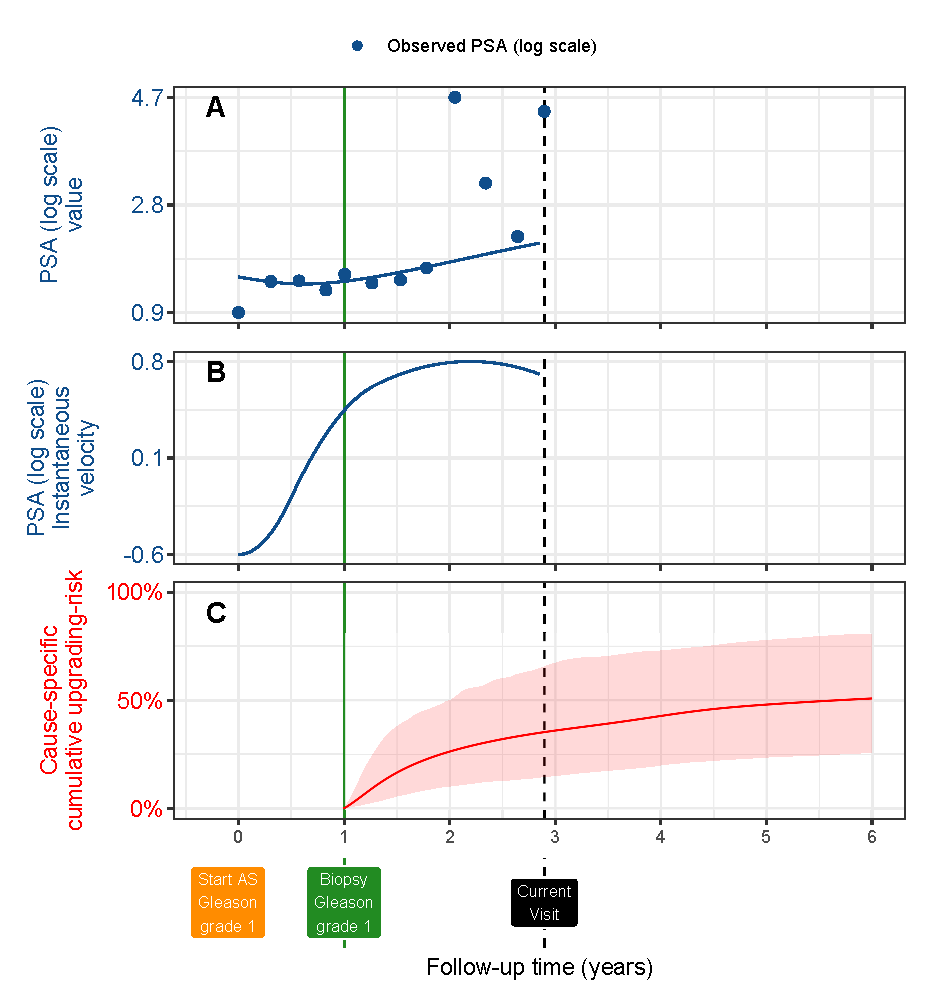
\includegraphics[width=\columnwidth]{images/jmExplanationPlot_113.eps}}
\caption{\textbf{Illustration of the joint model on a real PRIAS patient}. \textbf{Panel~A:} Observed PSA (blue dots) and fitted PSA (solid blue line), log-transformed. \textbf{Panel~B:} Estimated instantaneous velocity of PSA (log-transformed). \textbf{Panel~C}: Predicted cumulative-risk of upgrading (95\% credible interval shaded). Upgrading is defined as an increase in Gleason grade group from group~1 to 2 or higher. This risk of upgrading is available starting from the time of the latest negative biopsy (vertical green line at year 1 of follow-up). The joint model estimated it by combining the fitted value and fitted instantaneous velocity of PSA (log scale), and time of the latest negative biopsy. Black dashed line at year 3 denotes the time of current visit.}
\label{fig:jmExplanationPlot_113}
\end{figure}

\subsection{Model Validation}
We validated our PRIAS based risk prediction model internally in the PRIAS cohort, and externally using the largest five GAP3 database~\citep{gap3_2018} cohorts. These were, namely, University of Toronto AS (Toronto), Johns Hopkins AS (Hopkins), Memorial Sloan Kettering Cancer Center AS (MSKCC), King's College London AS (KCL), and Michigan Urological Surgery Improvement Collaborative AS (MUSIC). We assessed our model's ability to discriminate between patients who experience/do not experience upgrading, via the area under the receiver operating characteristic curve or AUC~\citep{rizopoulos2017dynamic}. We employed calibration plots~\citep{royston2013external,steyerberg2010assessing} and mean absolute risk prediction error~\citep{rizopoulos2017dynamic} to graphically and quantitatively evaluate the risk prediction accuracy of our model. Due to the longitudinal nature of AS studies, the AUC and prediction error varies over follow-up (Supplementary~B.1). Lastly, to resolve any potential model miscalibration in external GAP3 cohorts we aimed to recalibrate our model's baseline hazard of upgrading, individually for each GAP3 cohort (Supplementary~B.1).

\subsection{Personalized Schedules Web-Application}
We intend to utilize the predictions for cause-specific cumulative-risk of upgrading, to create personalized biopsy schedules for patients from both PRIAS and validation GAP3 cohorts. Subsequently, we aim to transform our model into a user friendly web-application including visualization of different biopsy risk thresholds and the consequence ( i.e dealy time???)